\subsubsection{2D compressible convection with a reference profile and material properties from BurnMan}
\label{sec:cookbooks-burnman}
\textit{This section was contributed by Juliane Dannberg and Ren{\'e} Gassm{\"o}ller}

In this cookbook we will set up a compressible mantle convection model that uses
the (truncated) anelastic liquid approximation (see Sections~\ref{sec:ala} and
\ref{sec:tala}), together with a reference profile read in from an ASCII data file.
The data we use here is generated with the open source mineral physics toolkit BurnMan
(\url{http://www.burnman.org}) using the python example program \texttt{simple\_adiabat.py}.
This file is available as a part of BurnMan, and provides a tutorial for how to generate
ASCII data files that can be used together with \aspect{}.
The computation is based on the Birch-Murnaghan equation of state, and uses a harzburgitic
composition. However, in principle, other compositions or equations of state can be used,
as long as the reference profile contains data for the reference temperature, pressure, density,
gravity, thermal expansivity, specific heat capacity and compressibility. Using BurnMan
to generate the reference profile has the advantage that all the material property data
are consistent, for example, the gravity profile is computed using the reference density.
\begin{figure}
  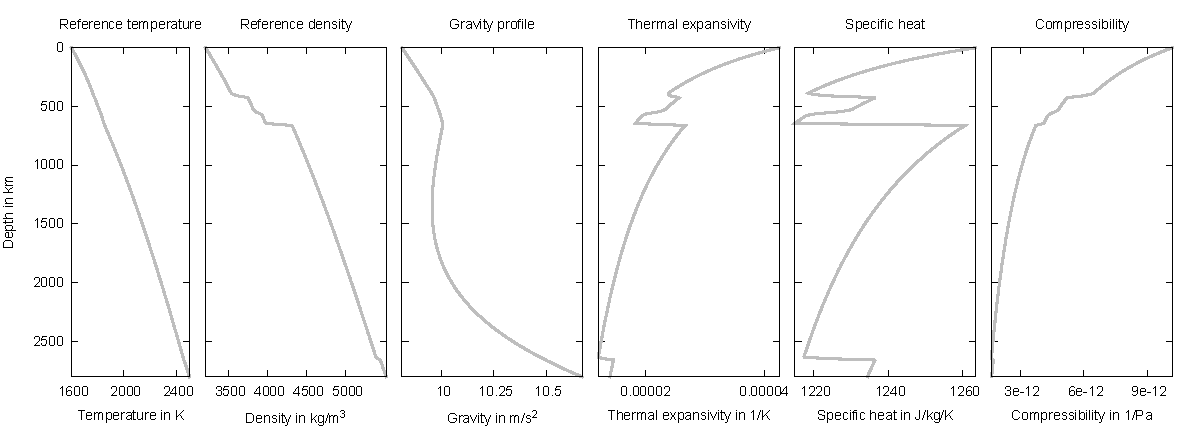
\includegraphics[width=\textwidth]{cookbooks/burnman/doc/reference_profile.pdf}
  \caption{\it Reference profile generated using BurnMan.}
  \label{fig:burnman-reference-profile}
\end{figure}
The reference profile is shown in Figure~\ref{fig:burnman-reference-profile}, and the corresponding data file
is located at \url{data/adiabatic-conditions/ascii-data/isentrope_properties.txt}.

\paragraph{Setting up the \aspect{} model.}
In order to use this profile, we have to import and use the data in the adiabatic conditions
model, in the gravity model and in the material model, which is done using the corresponding
ASCII data plugins. The input file is provided in \url{cookbooks/burnman/burnman.prm}, and it uses the
2d shell geometry previously discussed in Section~\ref{sec:shell-simple-2d} and surface velocities
imported from GPlates as explained in Section~\ref{sec:cookbooks-gplates}.

To use the BurnMan data in the material model, we have to specify that we want to use the
\texttt{ascii reference profile} model. This material model makes use of the functionality provided by
the \texttt{AsciiData} classes in \aspect{}, which allow plugins such as material models,
boundary or initial conditions models to read in ASCII data files (see for example Section~\ref{sec:geomio}).
Hence, we have to provide the directory and file name of the data to be used in the separate subsection
\texttt{Ascii data model}, and the same functionality and syntax will also be used for the
adiabatic conditions and gravity model.

The viscosity in this model is computed as the product of a profile $\eta_r(z)$, where $z$ corresponds to the depth direction of the chosen geometry model, and a
term that describes the dependence on temperature:
\begin{align*}
\eta(z,T) = \eta_r(z) \eta_0 \exp\left(-A \frac{T - T_{\text{adi}}}{T_{\text{adi}}}\right),
\end{align*}
where $A$ and $\eta_0$ are constants determined in the input file via the parameters
\texttt{Viscosity} and \texttt{Thermal viscosity exponent}, and $\eta_r(z)$ is a stepwise constant
function that determines the viscosity profile. This function can be specified by providing a list of
\texttt{Viscosity prefactors} and a list of depths that describe in which depth range each prefactor
should be applied, in other words, at which depth the viscosity changes. By default, it is set
to viscosity jumps at 150\,km depth, between upper mantle and transition zone,
and between transition zone and lower mantle). The prefactors used here lead to a low-viscosity
asthenosphere, and high viscosities in the lower mantle. To make sure that these viscosity jumps
do not lead to numerical problems in our computation (see Section~\ref{sec:sinker-with-averaging}),
we also use harmonic averaging of the material properties.
\lstinputlisting[language=prmfile]{cookbooks/burnman/doc/material_model.part.prm.out}
As the reference profile has a depth dependent density and also contains data for the compressibility,
this material model supports compressible convection models.

For the adiabatic conditions and the gravity model, we also specify that we want to use the respective
\texttt{ascii data} plugin, and provide the data directory in the same way as for the material
model. The gravity model automatically uses the same file as the adiabatic conditions model.
\lstinputlisting[language=prmfile]{cookbooks/burnman/doc/adiabatic_conditions.part.prm.out}
\lstinputlisting[language=prmfile]{cookbooks/burnman/doc/gravity_model.part.prm.out}

To make use of the reference state we just imported from BurnMan, we choose a formulation of the
equations that employs a reference state and compressible convection, in this case the anelastic
liquid approximation (see Section~\ref{sec:ala}).
\lstinputlisting[language=prmfile]{cookbooks/burnman/doc/formulation.part.prm.out}
This means that the reference profiles are used for all material properties in the model, except for
the density in the buoyancy term (on the right-hand side of the force balance equation~\eqref{eq:stokes-1},
which in the limit of the anelastic liquid approximation becomes Equation~\eqref{eq:stokes-ALA-1}).
In addition, the density derivative in the mass conservation equation
(see Section~\ref{sec:mass-conservation-approximation}) is taken from the adiabatic
conditions, where it is computed as the depth derivative of the provided reference density profile
(see also Section~\ref{sec:combined_formulations}).

\paragraph{Visualizing the model output.}
If we look at the output of our model (for example in \texttt{ParaView}), we can see how cold, highly
viscous slabs are subducted and hot plumes rise from the core-mantle boundary. The final time step of
the model is shown in Figure~\ref{fig:burnman-convection}, and the full model evolution can be found
at \url{https://youtu.be/nRBOpw5kp-4}.
Visualizing material properties such as density, thermal expansivity or specific heat shows how they
change with depth, and reveals abrupt jumps at the phase transitions, where properties change from one
mineral phase to the next. We can also visualize the gravity and the adiabatic profile, to ensure that
the data we provided in the \url{data/adiabatic-conditions/ascii-data/isentrope_properties.txt} file
is used in our model.

\begin{figure}
  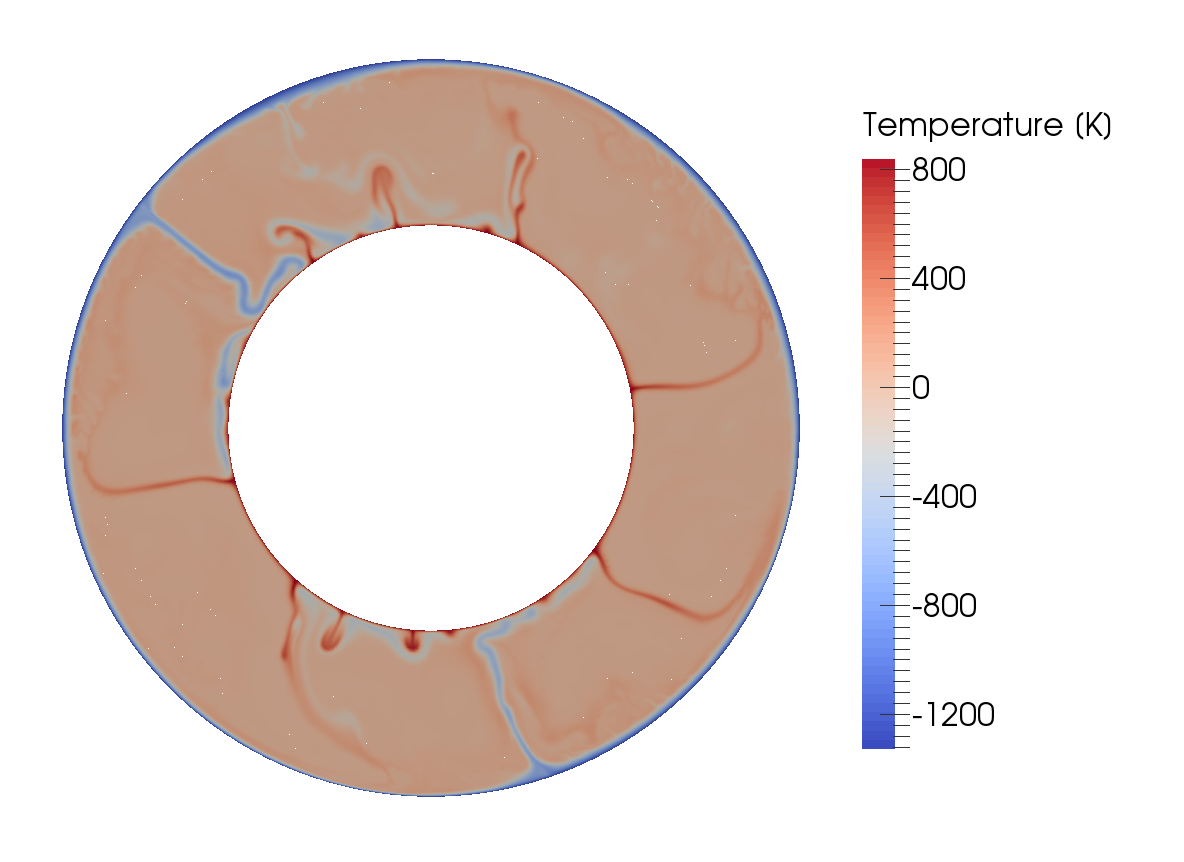
\includegraphics[width=0.48\textwidth]{cookbooks/burnman/doc/temperature.png}
  \hfill
  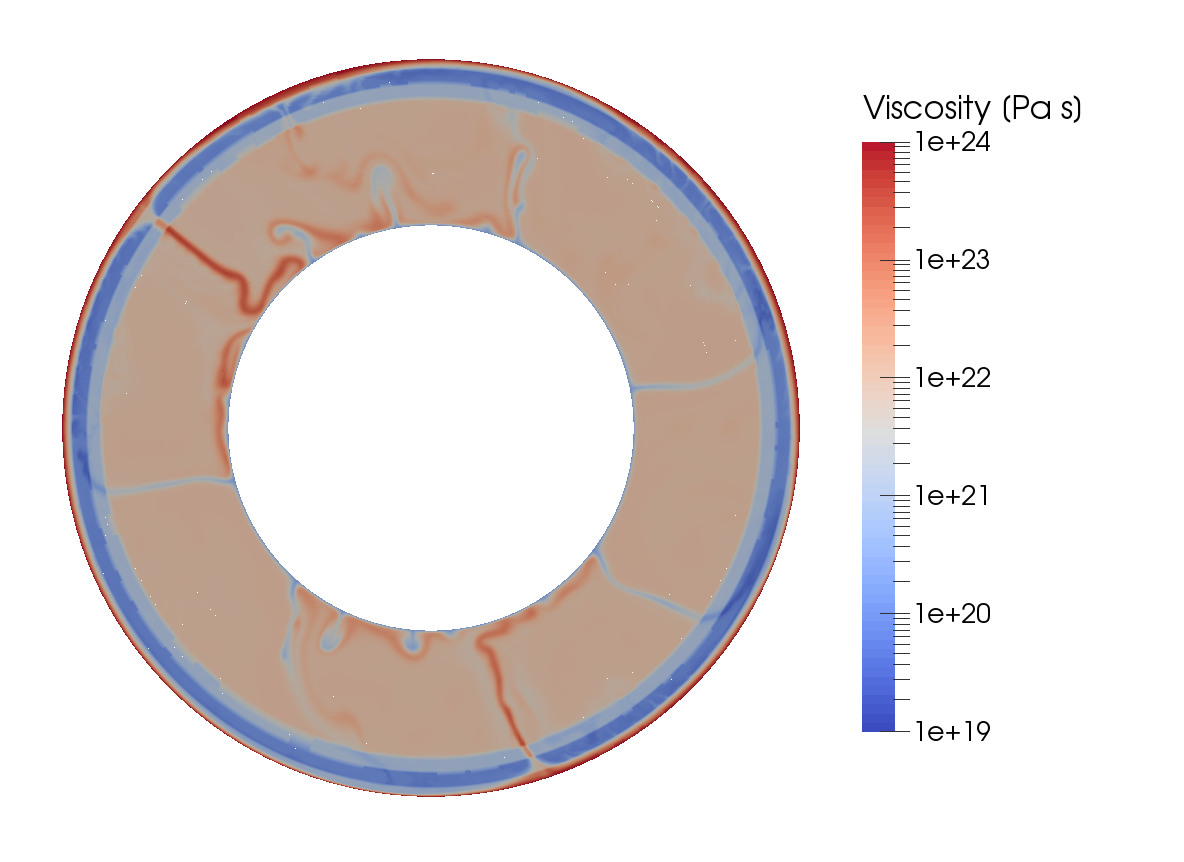
\includegraphics[width=0.48\textwidth]{cookbooks/burnman/doc/viscosity.png}
  \caption{\it Compressible convection in a 2d spherical shell, using a reference profile exported
               form BurnMan, which is based on the Birch-Murnaghan equation of state. The figure shows the
               state at the end of the model evolution over 260\,Ma.}
  \label{fig:burnman-convection}
\end{figure}

\paragraph{Comparing different model approximations.}
For the model described above, we have used the anelastic liquid approximation. However, one might want
to use different approximations that employ a reference state, such as the truncated anelastic liquid
approximation (TALA, see Section~\ref{sec:tala}), which is also supported by the
\texttt{ascii reference profile} material model. In this case, the only change compared to ALA
is in the density used in the buoyancy term, the only place where the temperature-dependent density
instead of the reference density is used. For the TALA, this density only depends on the temperature
(and not on the dynamic pressure, as in the ALA). Hence, we have to make this change in the appropriate
place in the material model (while keeping the formulation of the equations set to
\texttt{anelastic liquid approximation}):
\lstinputlisting[language=prmfile]{cookbooks/burnman/doc/tala.part.prm.out}

We now want to compare these commonly used approximations to the ``isothermal compression approximation''
(see Section~\ref{sec:ica}) that is unique to \aspect{}. It does not require a reference state and uses
the full density everywhere in the equations except for the right-hand side  mass conservation, where the
compressibility is used to compute the density derivative with regard to pressure.
Nevertheless, this formulation can make use of the reference profile computed by BurnMan and compute the
dependence of material properties on temperature and pressure in addition to that by taking into account
deviations from the reference profile in both temperature and pressure. As this requires a modification
of the equations outside of the material model, we have to specify this change in the
\texttt{Formulation} (and remove the lines for the use of TALA discussed above).
\lstinputlisting[language=prmfile]{cookbooks/burnman/doc/formulation_ica.part.prm.out}
As the ``isothermal compression approximation'' is also \aspect{}'s default for compressible models,
the same model setup can also be achieved by just removing the lines that specify which \texttt{Formulation}
should be used.

The Figures~\ref{fig:burnman-comparison} and \ref{fig:burnman-vrms} show a comparison between the different
models. They demonstrate that upwellings and downwellings may occur in slightly different places and at
slightly different times when using a different approximation, but averaged model properties describing
the state of the model -- such as the root mean square velocity -- are similar between the models.

\begin{figure}
\centering
  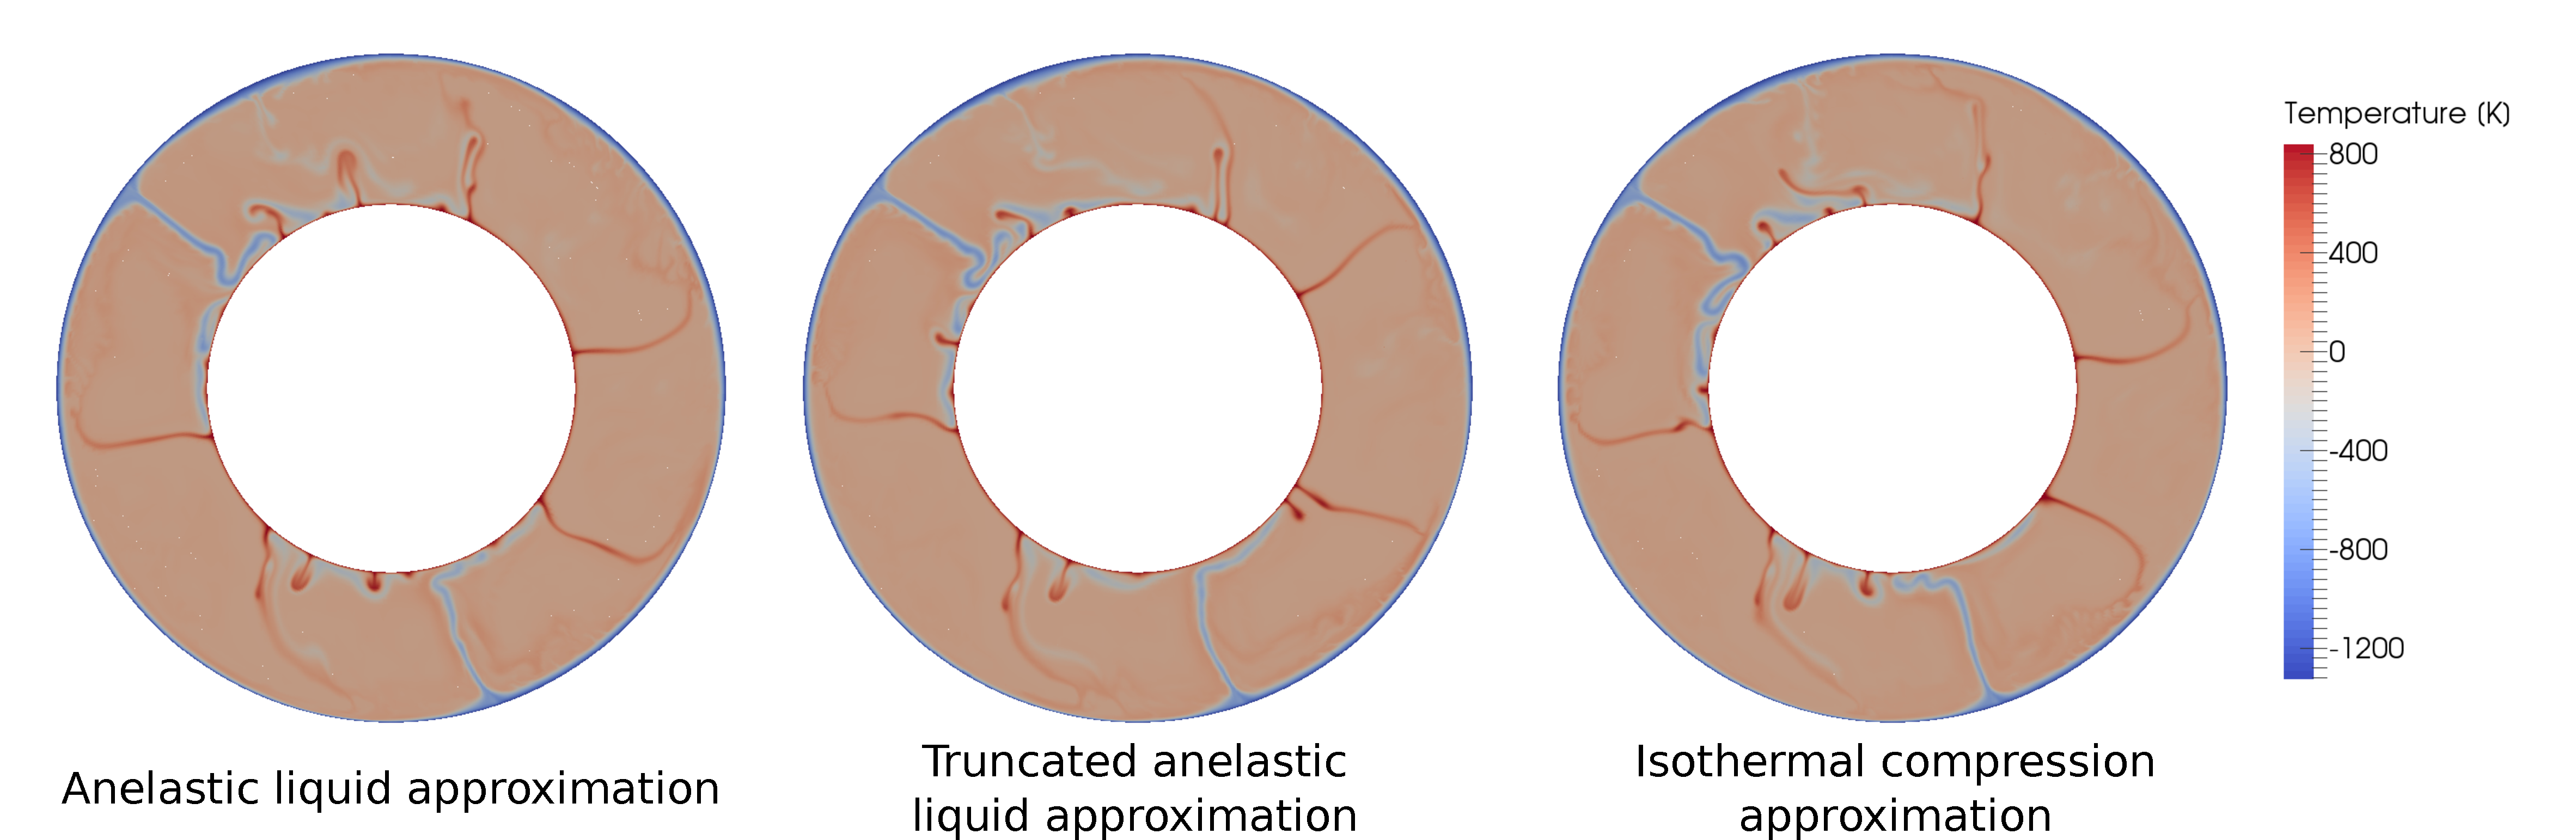
\includegraphics[width=0.95\textwidth]{cookbooks/burnman/doc/comparison.pdf}
  \caption{\it Comparison between the anelastic liquid approximation,
               the truncated anelastic liquid approximation
               and the isothermal compression approximation,
               showing the temperature distribution for the different models at
               the end of the model evolution at 260\,Ma.}
  \label{fig:burnman-comparison}
\end{figure}

\begin{figure}
\centering
  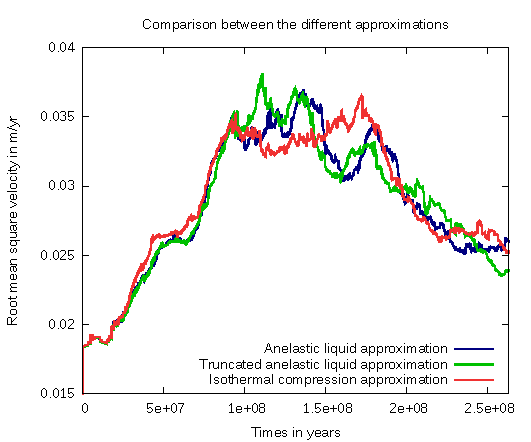
\includegraphics[width=0.5\textwidth]{cookbooks/burnman/doc/vrms.pdf}
  \caption{\it Comparison between the anelastic liquid approximation,
               the truncated anelastic liquid approximation
               and the isothermal compression approximation,
               showing the evolution of the root mean square velocity.}
  \label{fig:burnman-vrms}
\end{figure}
